\documentclass[12pt]{article}

\usepackage{amssymb,amsmath}
\usepackage[margin=1.0in]{geometry}
\usepackage{fancyhdr} % required for custom header
\usepackage{graphicx}
\usepackage{listings}
\usepackage{courier}
\usepackage{natbib}
\usepackage[usenames,dvipsnames]{color}

%set up the header
\pagestyle{fancy}
\lhead{Trever T. Hines}
\chead{RO 16-15 Reasearch Proposal}
\rhead{\today}

\setlength{\headheight}{15pt}
\renewcommand\headrulewidth{1.0pt} % Size of the header rule

%% Title
%%------------------------------------------------------------------------------
\title{	
 \rule{\headwidth}{1.0pt}
 Research proposal for RO 16-15:
 Novel crustal deformation models \
 characterizing earthquake hazard and its uncertainties in the western U.S.\
 \rule{\headwidth}{1.0pt}
 \author{Trever T. Hines}}

\begin{document}
\maketitle

\section*{Research Objective}

An accurate assessment of seismic hazard requires estimates of where faults have previously ruptured as well as the uncertainties on those estimates.  The research proposed here addresses the latter. Finite-fault rupture models, which are obtained through a regularized least squares inversion of geodetic data, lack meaningful quantifications of uncertainty. This is because model uncertainties are highly dependent upon the chosen regularization scheme and the degree to which that regularization is enforced, which is determined by a penalty parameter. There are statistically based methods for objectively choosing the penalty parameter \citep[e.g.][]{Yabuki1992,Fukuda2008}, but the choice of regularization scheme (e.g. imposing smallness or smoothness on the solution) is subjective and lacks physical justification.  Although regularization makes it difficult to assess the uncertainty in a solution, it is necessary for preventing solutions with magnitudes and directions of fault slip that are intuitively implausible. Since the motivation behind adding regularization is to ensure that rupture models are physically reasonable, the choice of regularization should be based on our understanding of how faults rupture.  In such case, regularization can be viewed as adding a prior constraint in a Bayesian sense. A posterior ensemble can then be found which provides a meaningful description of the range of plausible rupture models that are capable of describing the data.  My goal is to develop a method for imposing physically motivated prior constraints on finite-fault rupture models. I then plan to apply this method to the 2004 Parkfield earthquake.  

\subsection*{Prior Constraints}
I consider three well established, empirically derived relationships to use as prior constraints for rupture models. (1) Faults slip in the direction of maximum shear stress, $\sigma_\parallel$, \citep{Wallace1951}; (2) slip occurs when the Mohr-Coulomb failure criterion is exceeded \citep{Byerlee1978}; and (3) shear stress drop, $\Delta \sigma_\parallel$, tends to be in the range of 0.1 to 10 MPa, regardless of the spatial extent and magnitude of the earthquake \citep{Kanamori1975,Shearer2006}.  Constructing a prior based on the first two relationships would require an understanding of the ambient pre-seismic stress.  To constrain the direction on fault slip, only the orientation of the ambient stress needs to be known, which can be estimated from background seismicity.  The absolute ambient stress is necessary if I want to form a prior from the Mohr-Coulomb failure criterion, which states that
\begin{equation}\label{eq:MohrCoulomb}
  \mathbf{\sigma_\parallel} = C + \mu \mathbf{\sigma_\bot},
\end{equation}
where $\sigma_\bot$ is the normal stress on a fault, $C$ is cohesion, and $\mu$ is the coefficient of friction.  Barring earthquakes that produce significant stress overshoot, the shear stress drop at any point on a fault cannot exceed its frictional strength.  Additionally, the coseismic increase in shear stress along the edges of a rupture zone cannot exceed the frictional strength. In order to calculate the maximum shear stress for a strike-slip fault, I assume that the normal stress is primarily due to overburden.  Indirect inferences of the San Andreas fault strength which are based on heat flow and stress orientations across the fault find that $\mu\approx0.1$ \citep{Brune1969,Zoback1987}.  Laboratory experiments on gouge taken from the San Andreas fault find $\mu\approx0.3$ \citep{Carpenter2011}, while even higher values of 0.6 to 1.0 are suggested by \citet{Byerlee1978}. Even though the coefficient of friction can be debatable, I only need a reasonable upper bound on $\mu$ in order to limit the maximum shear stress drop in a rupture model.  Assuming no cohesion and $\mu\approx0.3$, the shear stress required for an earthquake is on the order of 100 MPa.  Therefore a rupture model should satisfy the condition $|\Delta\sigma_\parallel|\lesssim 100$ MPa everywhere on a fault.  This can then be used to constrain $\Delta u$ through the relationship
\begin{equation}\label{eq:StressSlip}
  \Delta \sigma_\parallel (\xi_1) = \int_F K(\xi_1,\xi_2) \Delta u(\xi_2) d\xi_2,
\end{equation}
where $K(\xi_1,\xi_2)$ describes the stress drop at $\xi_1$ resulting from slip at $\xi_2$, and $F$ denotes the fault.  When assuming that our domain is a homogeneous, isotropic, elastic, half-space, $K$ can be computed with the analytical solution from \citet{Okada1992}.  

The observation that stress drop is consistently on the order of 0.1 to 10 MPa offers a tighter constraint on fault slip than the Mohr-Coulomb failure criterion.  Seismologically determined stress drop can be interpreted as the average coseismic change in shear stress over the rupture zone.  The difficulty is that the rupture zone is not known \textit{a priori}, since that is what I am trying to estimate in a finite-fault rupture model.  However, it is known that stress drop is invariant to the spatial extent of the earthquake and thus I can posit that the stress drop at each point on a ruptured fault should also be subject to the same bounds of 0.1 to 10 MPa.  Outside of the rupture zone, stress drop will generally be negative (i.e. pushed closer to failure).  When considering the entire fault, not just the area that ruptured, I can then impose an upper bound of 10 MPa on $\Delta \sigma_\parallel$.  \citet{Sun2011} also explored coseismic inversions with constraints on stress drop.  Their model assumed that stress drop must be uniform over the proposed fault geometry.   In contrast, I am merely imposing an upper limit on stress drop, which allows for a greater deal of flexibility in our solution.        

\subsection*{Synthetic Demonstration}
I use a synthetic test to demonstrate how effectively these physical constraints regularize finite-fault rupture models.  A thoroughly annotated IPython notebook containing all the work done for this synthetic test can be found in www.github.com/treverhines/ MendenhallProposal.git.  In this synthetic test, I invert displacements resulting from slip on an infinitely long, strike-slip fault embedded in a homogeneous, elastic half-space.  This degenerates to a two-dimensional problem where the fault strike and displacements are in the anti-plane direction.  The fault extends from the surface to 15 km depth and is discretized into 10 segments. I impose slip which is consistent with a uniform stress drop of 5 MPa.  The slip and resulting displacements, with added noise, are shown in Figure 1.

Inverting surface displacements for fault slip is typically done by using regularized least squares to solve
\begin{equation}\label{eq:Forward}
  u(x) = \int_F G(x,\xi) \Delta u(\xi) d\xi,
\end{equation}
where $u(x)$ are the observable coseismic surface displacements, and $G(x,\xi)$ describes displacements at $x$ resulting from slip at $\xi$.  For this two-dimensional problem, the maximum shear stress is in the anti-plane direction and $\Delta u$ can be forced to be in the same direction by solving eq. \ref{eq:Forward} with a bounded least squares algorithm \citep{Lawson1995}.  If I wish to solve eq. \ref{eq:Forward} with constraints on $\Delta \sigma_\parallel$ rather than $\Delta u$, then the inverse of eq. \ref{eq:StressSlip} can be combined with eq. \ref{eq:Forward}, and then that equation can be solved with bounded least squares. I seek to put constraints on both $\Delta u$ and $\Delta \sigma_\parallel$, and there is no immediately apparent way to impose such constraints with bounded least squares. I then resort to the more expensive, although more informative, Monte Carlo methods.  Specifically, I use a Metropolis-Hastings algorithm to estimate $\Delta u$ with the prior constraint that $\Delta u$ is positive and $\Delta \sigma_\parallel < 10$ MPa for each fault segment. I also add a prior constraint on the seismic potency, which I define for this two-dimensional problem as the average slip multiplied by the fault width.  The seismic potency for the true model is 0.58 $\mathrm{km}^2$ and I use a normally distributed prior with a mean of 0.6 $\mathrm{km}^2$ and standard deviation of 0.1 $\mathrm{km}^2$.  

For each iteration in the Metropolis-Hastings algorithm, the likelihood of a trial model is calculated based on how well it agrees with our prior and how well it agrees with the observed data.  If I have $N$ observations and $M$ unknown model parameters, then the computational cost of comparing the predictions of the trial model to the observed data is $O(NM)$. The cost of testing if a trial model agrees with our prior is $O(M^2)$, where the main burden is in evaluating eq. \ref{eq:StressSlip} to ensure that stress drop is within our prior bounds.  However, the discretized matrix representing $K$ is sparse because stress drop on a fault segment is mostly a function of slip on nearby fault segments.  If I take advantage of this sparsity then the cost of comparing a test model to the prior is $O(M)$.  Thus, the main bottleneck in our algorithm is in comparing the observations to the predictions for each trial model.  

\begin{figure}
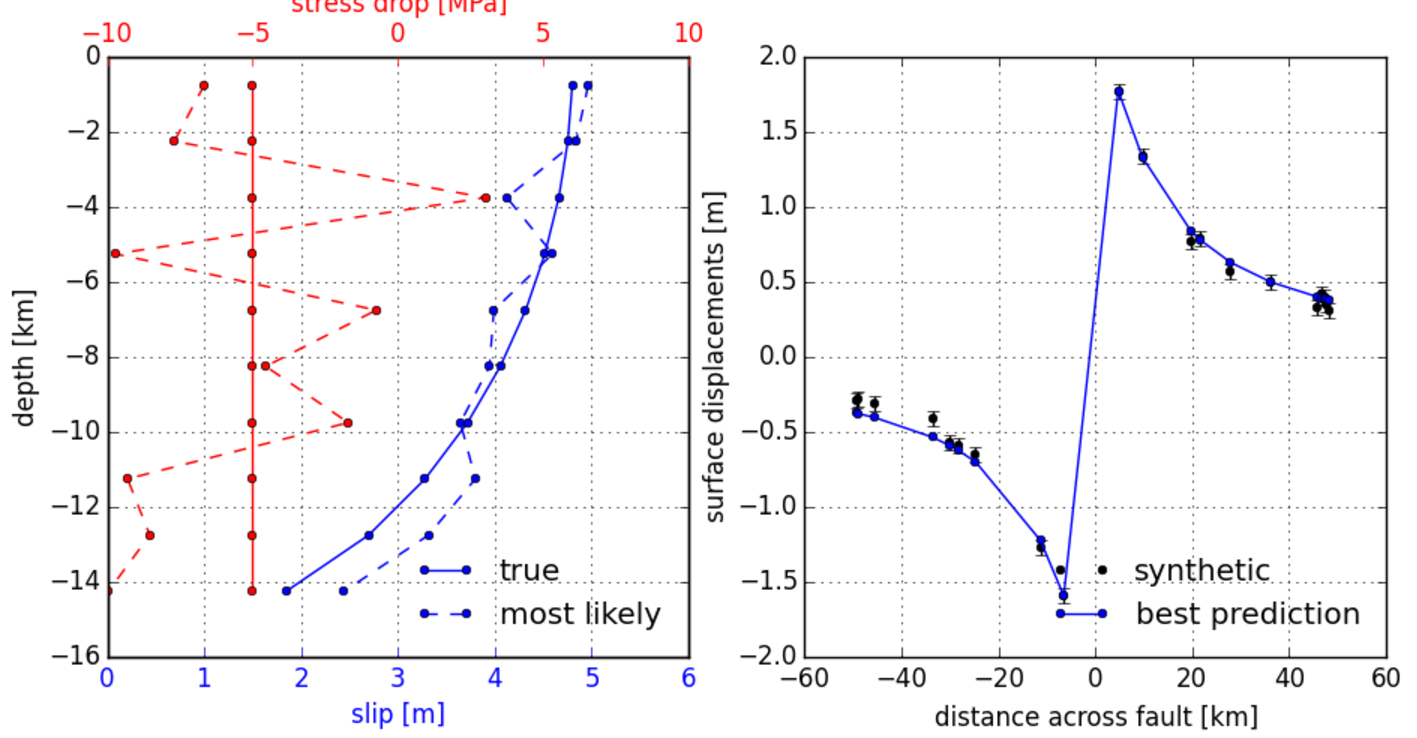
\includegraphics[width=1.0\textwidth]{figure_1}
\caption{Left: solid blue and red lines indicates the true slip and stress drop respectively, and dashed lines indicate the inferred slip and stress drop for the most likely posterior model.  Right: synthetic data with their 68\% confidence intervals are shown as black points, and the blue line is the prediction from the most likely posterior model.}  
\end{figure}

I ran one million iterations of the Metropolis-Hastings algorithm, which takes about one minute on a desktop computer.  Our most likely slip model is shown in Figure 1 along with the predicted displacements.  The marginal posterior distributions of slip are shown in the left panel of Figure 2.  For comparison I ran another inversion without bounds on stress drop, and the marginal posteriors are shown in the right panel in Figure 2.  When stress drop is unbounded, most of the retained models have no slip on all but a few fault segments, which then have 10s of meters of slip in order to produce the required potency.  As a result, the posterior slip distributions tend to be wide and have low mean values.  This is in sharp contrast to the posterior slip distributions when stress drop is bounded.  In that case, the posteriors have mean values that closely match the true slip model.   

\begin{figure}
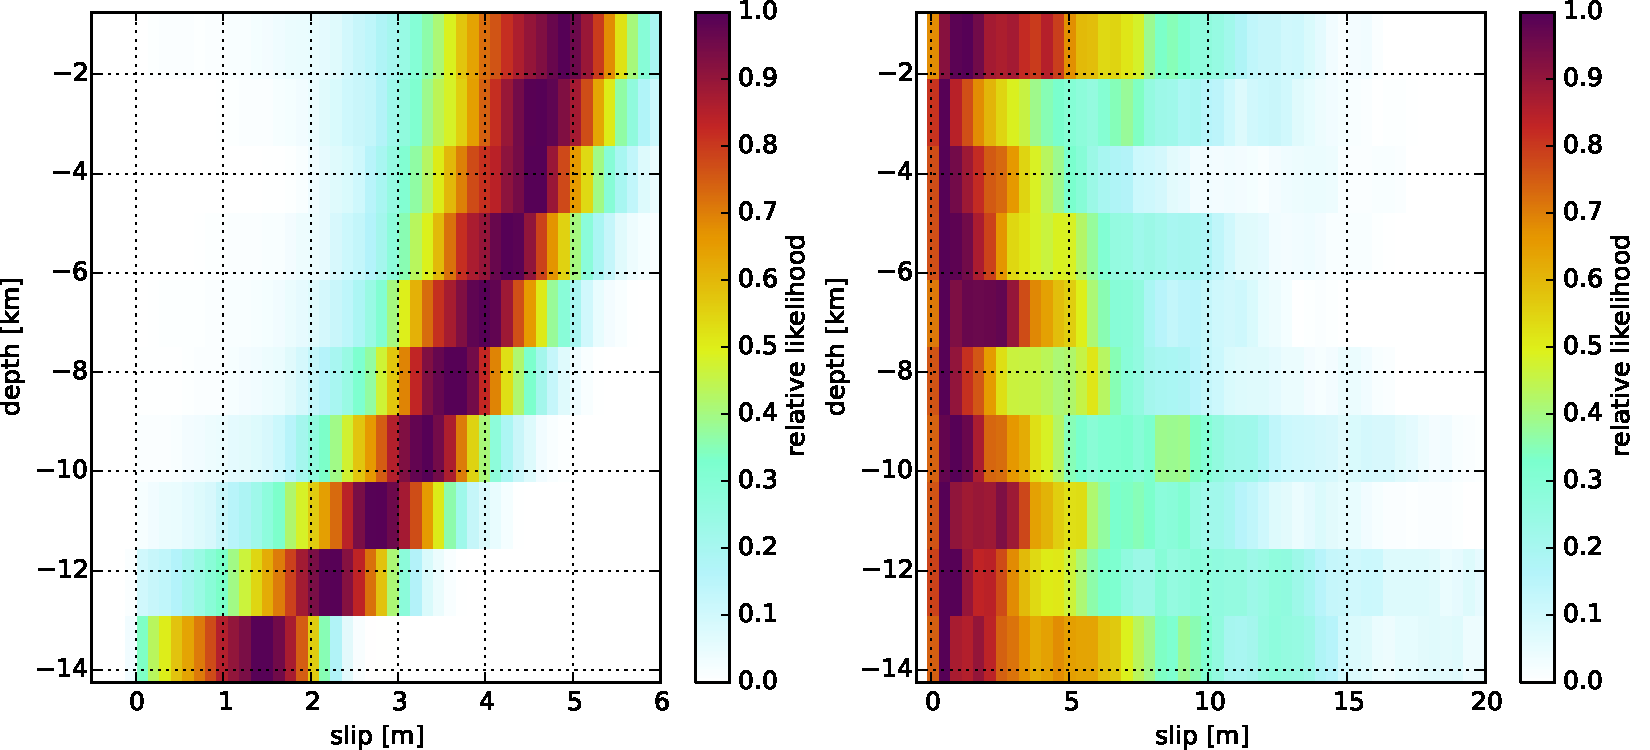
\includegraphics[width=1.0\textwidth]{figure_2}
\raggedleft
\caption{Left: marginal posterior probability density function of slip for each depth interval when stress drop is bounded to be less than 10 MPa (left) and when stress is unbounded (right).}  
\end{figure}

\subsection*{2004 Parkfield Earthquake}
The 2004 Parkfield earthquake is well suited for the Bayesian coseismic slip inversion proposed here.  Coseismic displacements for this earthquake were recorded at about a dozen ideally positioned, continuous GPS stations. InSAR and campaign GPS can also be used to estimated coseismic displacements although it is difficult to definitively discern coseismic from postseismic displacements \citep{Johanson2006}. Nonetheless, all of the data that I can potentially use to measure coseismic displacements have been made readily available through UNAVCO.  In addition to the wealth of geodetic data, the geometry of the Parkfield segment of the San Andreas fault is well known \citep{Simpson2006}.  This allows us to circumvent the computationally expensive task of trying to simultaneously estimate the fault geometry with the distribution of fault slip \citep[e.g.][]{Fukuda2008}. 

Revisiting the Parkfield earthquake from a Bayesian perspective could also have implications for assessing seismic hazard.  In particular, if we know where the San Andreas fault ruptured during the earthquake and we have a good understanding of the uncertainties on the rupture model, then we can better quantify our confidence in where we believe slip deficits exist \citep{Murray2006}.  Although \citet{Page2009} did attempt to address the question of uncertainty in coseismic slip estimates for the 2004 Parkfield earthquake, their estimates of uncertainty were based upon slip inversions with Laplacian smoothing.  I believe that an accurate estimate of uncertainty in finite-fault rupture models requires the use of a Bayesian inverse method with physically motivated prior constraints.

\section*{Work Plan}
The first stage of my project will be focused on code development and synthetic testing.  With the success of the two-dimensional synthetic test, the next step is to extend the Bayesian inverse method with physically motivated priors into three-dimensions.  While there are additional geometric considerations, the transition to three-dimensions should be fairly straight forward, although the computational costs will likely become a limiting factor due to the larger model space.  Three-dimensional, static coseismic slip models typically have a couple hundred model parameters.  This may be too large of a mode space to feasibly search with the standard Metropolis-Hastings algorithm that I used in the synthetic test.  Instead, I will likely need to use a more efficient algorithm such as CATMIP \citep{Minson2013}.  Based on the synthetic tests in \citep{Minson2013}, I would need to evaluate the forward problem on the order of $10^{8}$ times to adequately sample my posterior.  This may take a few hours to run on a single CPU, which is certainly tractable.  I will perform numerous synthetic coseismic slip inversions as a means of validation for this inverse method as well as to build intuition on how the priors are influencing the posterior solutions.

The second stage for this project will be to apply this inverse method to the 2004 Parkfield earthquake.  The continuous GPS data for this earthquake is available at UNAVCO and is immediately ready to use.  The campaign GPS and InSAR data are also available through UNAVCO, although they are in their raw data format and need to be run through processing software. Once the data is compiled, performing the coseismic inversion should be straight forward.        

\section*{Anticipated Expenses}
The proposed research will require a significant amount of computation time.  I will need a desktop (${\sim}\$1,000$) for code developement and small scale simulations and inversion.  For high performance computing needs, I will apply for a cluster allocation through the Extreme Science and Engineering Discovery Environment (EXSEDE), which has no cost.  I will use Python for all of my data analysis and Pylith \citep{Aagaard2013} to compute Green's functions in cases where analytical solutions are unavailable, both of which are free and open source.  Additional expenses will include travel for conferences (${\sim}\$2,000$ per year) and publication fees (${\sim}\$1,000$).  



%\bibliography{mybib}{}
%\bibliographystyle{plain}
\bibliographystyle{apalike}
\bibliography{mybib}

\end{document}